\clearpage

\section{Pulse Shaper}

\begin{tcolorbox}	
	\begin{tabular}{p{2.75cm} p{0.2cm} p{10.5cm}} 	
		\textbf{Header File}   &:& pulse\_shaper.h \\
		\textbf{Source File}   &:& pulse\_shaper.cpp \\
	\end{tabular}
\end{tcolorbox}

This block applies an electrical filter to the signal. It accepts one input signal that is a sequence of Dirac delta functions and it produces one output signal continuous in time and in amplitude.

\subsection*{Input Parameters}

\begin{table}[h]
	\centering
	\begin{tabular}{|c|c|p{60mm}|c|ccp{60mm}}
		\cline{1-4}
		\textbf{Parameter} & \textbf{Type} & \textbf{Values} &   \textbf{Default}& \\ \cline{1-4}
		filterType & string & RaisedCosine, Gaussian & RaisedCosine \\ \cline{1-4}
		impulseResponseTimeLength & int & any & $16$ \\ \cline{1-4}
		rollOfFactor & real & $\in \left[0,1\right]$ & $0.9$ \\ \cline{1-4} 
	\end{tabular}
	\caption{Pulse shaper input parameters}
	\label{table:pulse_shaper_in_par}
\end{table}

%\begin{itemize}
%	\item filterType\{RaisedCosine\} \linebreak
%	\item impulseResponseTimeLength\{16\}\linebreak (int) 
%	\linebreak (This parameter is given in units of symbol period)
%	\item rollOfFactor\{0.9\} \linebreak
%	(real $\in$ [0,1])
%\end{itemize}

\subsection*{Methods}

PulseShaper(vector$<$Signal *$>$ \&InputSig, vector$<$Signal *$>$ OutputSig) :FIR$\_$Filter(InputSig, OutputSig)\{\};
\bigbreak	
void initialize(void);
\bigbreak	
void setImpulseResponseTimeLength(int impResponseTimeLength)
\bigbreak
int const getImpulseResponseTimeLength(void)
\bigbreak	
void setFilterType(PulseShaperFilter fType)
\bigbreak
PulseShaperFilter const getFilterType(void)
\bigbreak	
void setRollOffFactor(double rOffFactor)
\bigbreak
double const getRollOffFactor()

\subsection*{Functional Description}

The type of filter applied to the signal can be selected trough the input parameter \textit{filterType}. Currently the only available filter is a raised cosine.

The filter's transfer function is defined by the vector \textit{impulseResponse}. The parameter \textit{rollOfFactor} is a characteristic of the filter and is used to define its transfer function.

\subsection*{Input Signals}

\subparagraph*{Number}: 1

\subparagraph*{Type}: Sequence of Dirac Delta functions (ContinuousTimeDiscreteAmplitude)

\subsection*{Output Signals}

\subparagraph*{Number}: 1

\subparagraph*{Type}: Sequence of impulses modulated by the filter (ContinuousTimeContinuousAmplitude)

\subsection*{Example}

\begin{figure}[h]
	\centering
	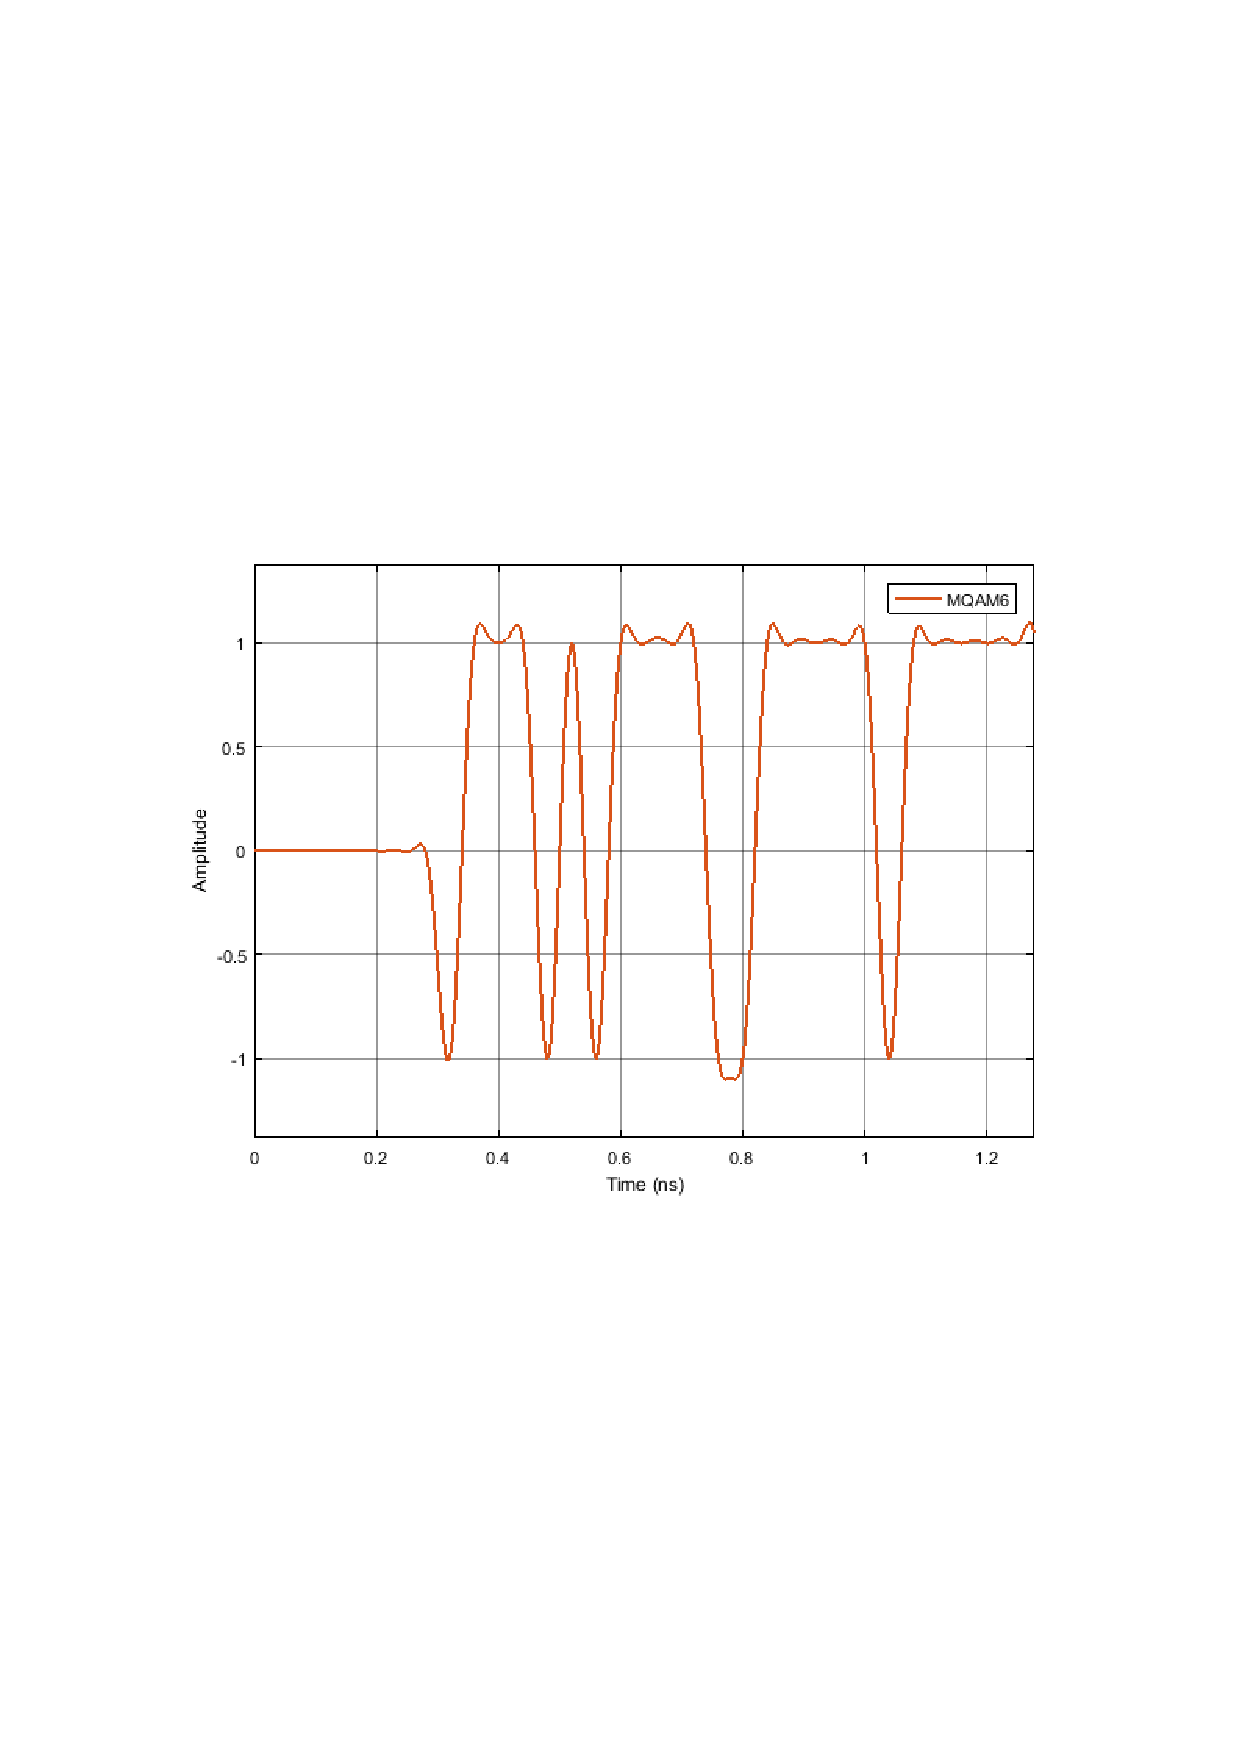
\includegraphics[clip, trim=0.5cm 9cm 0.5cm 9cm, width=\textwidth]{./lib/pulse_shaper/figures/MQAM_pulse_shaper_output.pdf}
	\label{MQAM6_DeterministicAppendZeros}\caption{Example of a signal generated by this block for the initial binary signal 0100...}
\end{figure}

\subsection*{Sugestions for future improvement}

Include other types of filters.
